% ============================================================================
% GALOSH — IEEE Signal Processing Letters version (4 pages + 1 reference page)
% Condensed from the arXiv manuscript; full tables/speed study stay in arXiv.
% Build: tectonic galosh_spl.tex
% ============================================================================
\documentclass[journal]{IEEEtran}
\usepackage{booktabs}
\usepackage{graphicx}
\usepackage{amsmath,amssymb}
\usepackage[hidelinks]{hyperref}

\begin{document}

\title{GALOSH: Blind, Training-Free Denoising of Raw Bayer and sRGB Images by
Parallel-Friendly Local Shrinkage}

\author{Yoshiro~Sato%
\thanks{A U.S. provisional patent application covering the methods described
herein has been filed (App.\ No.\ 64/058,343, 6 May 2026).}%
\thanks{Code and reproducible benchmarks:
\texttt{https://github.com/luxgrain/GALOSH}. An extended version with the full
per-dataset tables, per-ISO breakdowns, and the speed study is available as an
arXiv preprint~\cite{galosharxiv}.}}

\maketitle

\begin{abstract}
Classical training-free denoisers such as BM3D and non-local means owe much of
their strength to \emph{search}: content-dependent block matching that
parallelizes poorly and precludes fixed-latency implementations. We present
GALOSH (Generalized Anscombe LOcal SHrinkage), a search-free redesign: a blind
per-image Poisson--Gaussian noise fit, a generalized Anscombe transform, a
two-pass local Walsh--Hadamard shrinkage of luminance, and a luminance-guided
local regression of chrominance --- two deliberately different operators for
the two perceptually different noise components. Every stage is local,
data-independent, and regular; one core serves raw Bayer mosaics and sRGB/YUV
images. On four real-noise benchmarks (SIDD Medium and RawNIND, raw and sRGB)
GALOSH is consistently the strongest among the tested blind, training-free
methods --- surpassing BM3D- and NLM-family baselines even given an oracle
noise level --- while running $7\times$--$650\times$ faster than trained
baselines on the same GPU and practically on plain CPUs. The fixed structure
is designed to map onto fixed-point streaming hardware, supported by a working
INT16 realization.
\end{abstract}

\begin{IEEEkeywords}
Image denoising, blind denoising, variance stabilization, Walsh--Hadamard
transform, fixed-point arithmetic.
\end{IEEEkeywords}

\section{Introduction}
\IEEEPARstart{T}{wo} families dominate image denoising. Classical
training-free methods --- BM3D~\cite{bm3d} and non-local means~\cite{nlm} ---
need no data and generalize across sensors, but they assume a known noise
level and buy their quality with content-dependent \emph{search}: block
matching and neighborhood weighting whose irregular memory access and
data-dependent control flow resist vectorization, GPU occupancy, and any
fixed-latency budget. Learned methods reach excellent quality in the domain
they were trained on, but need training pairs, carry tens-of-thousands of MACs
per pixel, and degrade --- sometimes catastrophically --- outside their
training distribution, which we also observe. Beyond BM3D/NLM, the classical
family includes low-rank patch models (WNNM~\cite{wnnm}), patch-prior
optimization (EPLL~\cite{epll}), learned dictionaries (K-SVD~\cite{ksvd}), and
the blind Noise Clinic pipeline~\cite{noiseclinic}; these are likewise search-
or optimization-heavy, and we adopt BM3D/NLM --- with their CFA-aware and
color variants --- as the strongest widely-reproduced representatives.

This letter asks how much of the classical family's quality survives when the
search is removed \emph{by design}. GALOSH answers with a pipeline in which
every stage is local, regular, and data-independent: the noise model is
estimated blindly from the image itself~\cite{foi}; a generalized Anscombe
transform (GAT) makes a single global threshold valid everywhere; luminance is
denoised by two-pass local shrinkage on a Walsh--Hadamard decomposition
(a BayesShrink pilot~\cite{bayesshrink} followed by an empirical Wiener pass,
as in BM3D's two-step architecture); and chrominance by a luminance-guided
local linear regression (LOESS~\cite{loess} with a bilateral kernel, in the
guided/joint-bilateral tradition~\cite{kopf,guidedfilter}). The luma/chroma
split is deliberate: luminance noise reads as grain and coexists with texture,
whereas chroma noise reads as color blotches that are never acceptable, so the
two paths use different operators at different aggressiveness with independent
strength controls. The same core serves two thin front-ends:
\textbf{GALOSH-RAW} on the Bayer mosaic (a $2{\times}2$ Walsh--Hadamard
transform of each quad provides the luma/chroma split) and
\textbf{GALOSH-YUV/RGB} on rendered sRGB images (a linear-light BT.709
transform provides it). Our claim is not any single component but their
composition into a search-free, fully blind, two-domain pipeline whose
computation graph is fixed for every pixel of every image.

\section{Method}
\subsection{Shared core}
\paragraph{Blind noise estimation} The Poisson--Gaussian model
$\mathrm{Var}[x]=\alpha\,\mathbb{E}[x]+\sigma^2$ is fitted from the noisy
frame alone by a robust regression of local Laplacian variance against local
mean over overlapping blocks (a Foi-style estimator~\cite{foi}), yielding
per-image $(\alpha,\sigma^2)$ without calibration data or oracles.

\paragraph{Variance stabilization} The GAT
$f(x)=\tfrac{2}{\alpha}\sqrt{\alpha x+\tfrac{3}{8}\alpha^2+\sigma^2}$ maps the
signal-dependent noise to approximately unit variance, so one global threshold
is valid across the frame; the exact unbiased inverse~\cite{makitalo} is
applied on output. Channel-wise median absolute deviation of high-pass
residuals supplies the residual scale.

\paragraph{Luminance: two-pass local shrinkage (LOSH)} Luminance is denoised
on overlapping $8{\times}8$ Walsh--Hadamard blocks under stride-1 cycle
spinning: pass~1 builds a pilot with a robust BayesShrink
threshold~\cite{bayesshrink}; pass~2 applies empirical Wiener gains computed
from the pilot's coefficients; overlapping blocks are recombined by windowed
overlap-add. This replaces BM3D's collaborative 3-D stack over
\emph{searched} blocks with a dense cycle-spun local transform --- the one
move that removes all content dependence.

\paragraph{Chrominance: luminance-guided regression} Each chroma plane is
denoised by a first-order locally weighted regression on the denoised
luminance (a Y-guided LOESS~\cite{loess} with a bilateral kernel, equivalent
in spirit to guided filtering~\cite{guidedfilter,kopf}): within each window,
kernel weights combine spatial distance and luminance similarity, and the
MAP-regularized slope/intercept re-color the luminance structure. A
multi-scale residual pyramid extends the same operator to coarse blotches.
Re-assembled chroma is clamped to the local input chroma range (``a denoiser
must not invent colors absent from its input''). The two paths expose
independent strengths $s_L,s_C$; all benchmarks use fixed defaults.

\subsection{Domain front-ends}
\paragraph{GALOSH-RAW} operates directly on the Bayer mosaic: after the blind
fit and GAT, a CFA-adapted achromatic dark reference (IRLS estimate of the
achromatic floor) is subtracted, and a stride-1 cycle-spun $2{\times}2$
Walsh--Hadamard transform maps each Bayer quad to one full-resolution
luminance plane and three half-resolution chroma planes. Chroma is denoised at
half resolution, then returned to full resolution by a luminance-guided
joint-bilateral EWA-jinc upsampling with an anti-ringing clamp to the local
$2{\times}2$ input hull. The inverse WHT, dark restoration, and exact inverse
GAT yield a denoised Bayer frame for any downstream demosaicer.

\paragraph{GALOSH-YUV/RGB} accepts rendered sRGB: inverse gamma to linear
light, full-range BT.709 YCbCr; Y takes GAT + the two-pass LOSH (rendered
noise remains signal-dependent through the tone curve, which the GAT absorbs
to first order), Cb/Cr take the guided regression at full resolution; the same
local chroma-range clamp applies and the output is clamped to $[0,1]$.

\section{Experiments}
\paragraph{Setup} Raw domain: \textbf{SIDD Medium}~\cite{sidd} (80
full-resolution smartphone Bayer frames) and \textbf{RawNIND}~\cite{rawnind}
(1493 cross-camera $512^2$ real-noise crops). sRGB domain: the sRGB renditions
of the same sets (SIDD at full ${\sim}15.8$\,MP frames). \emph{Everything
runs blind}: no clean/noisy pairs, no per-image noise oracle; classical
baselines estimate $\sigma$ from the input, GALOSH uses its own blind fit, and
learned baselines use their published real-noise weights. Fidelity
(PSNR/SSIM) is computed in each native domain and perceptual metrics
(LPIPS~\cite{lpips}) on sRGB; on full-frame sRGB the learned baselines run
tiled inference and LPIPS is the mean over the same $1024^2$ tile grid for
every method --- a uniform protocol imposed by memory and metric limits at
that resolution. Baselines are domain-appropriate by design: CFA-capable
methods on raw (BM3D-CFA, NLM-CFA, their VST-front-end ablations, and the
raw-trained Blind2Unblind~\cite{b2u}); color-image methods on sRGB (CBM3D,
colored NLM, a self-guided filter, and the sRGB-trained NAFNet~\cite{nafnet},
Restormer~\cite{restormer}, SCUNet~\cite{scunet}).

\begin{table}[t]
\centering
\caption{Raw-domain blind denoising. All methods blind; bold /
\underline{underline} = best / 2nd among the blind, training-free methods;
Blind2Unblind is a trained upper reference. Full tables with DISTS/NIQE and
per-image times: extended version~\cite{galosharxiv}.}
\label{tab:raw}
\setlength{\tabcolsep}{3pt}
\footnotesize
\begin{tabular}{l ccc ccc}
\toprule
 & \multicolumn{3}{c}{SIDD Medium (80 full frames)} & \multicolumn{3}{c}{RawNIND (1493 crops)}\\
\cmidrule(lr){2-4}\cmidrule(lr){5-7}
Method & PSNR$\uparrow$ & SSIM$\uparrow$ & LPIPS$\downarrow$ & PSNR$\uparrow$ & SSIM$\uparrow$ & LPIPS$\downarrow$\\
\midrule
GALOSH FP32   & \textbf{48.13} & \textbf{0.9883} & \textbf{0.2030} & \underline{30.49} & \underline{0.7908} & \textbf{0.2395}\\
GALOSH INT16  & \underline{47.42} & \underline{0.9881} & \textbf{0.2030} & 30.17 & 0.7860 & \underline{0.2453}\\
VST+GALOSH    & 44.35 & 0.9765 & 0.2132 & \textbf{30.63} & \textbf{0.8163} & 0.2481\\
VST+BM3D-CFA  & 45.96 & 0.9851 & 0.2932 & 30.07 & 0.7792 & 0.4320\\
VST+NLM-CFA   & 40.36 & 0.9679 & 0.4048 & 29.03 & 0.7649 & 0.5452\\
BM3D-CFA      & 46.74 & 0.9862 & 0.2725 & 30.28 & 0.7848 & 0.4268\\
NLM-CFA       & 42.32 & 0.9729 & 0.3791 & 29.54 & 0.7735 & 0.5190\\
\midrule
Blind2Unblind & 49.07 & 0.9924 & 0.1169 & 30.68 & 0.7932 & 0.2215\\
\bottomrule
\end{tabular}
\end{table}

\begin{table}[t]
\centering
\caption{sRGB-domain blind denoising on SIDD Medium sRGB (80 scenes, full
${\sim}15.8$\,MP frames). Trained networks are an upper reference (NAFNet and
Restormer are trained \emph{on} SIDD).}
\label{tab:srgb}
\setlength{\tabcolsep}{4pt}
\footnotesize
\begin{tabular}{l ccc}
\toprule
Method & PSNR$\uparrow$ & SSIM$\uparrow$ & LPIPS$\downarrow$\\
\midrule
Noisy input     & 25.69 & 0.424 & 0.790\\
GALOSH-YUV      & \textbf{35.01} & \textbf{0.837} & \textbf{0.314}\\
CBM3D           & 27.09 & 0.492 & 0.721\\
Color-NLM       & \underline{28.92} & \underline{0.656} & \underline{0.534}\\
Guided filter   & 27.43 & 0.523 & 0.687\\
\midrule
NAFNet-SIDD     & 41.94 & 0.942 & 0.167\\
Restormer-SIDD  & 40.94 & 0.935 & 0.181\\
SCUNet-real     & 36.09 & 0.902 & 0.252\\
\bottomrule
\end{tabular}
\end{table}



\paragraph{Raw domain} Table~\ref{tab:raw}: among the tested blind,
training-free methods GALOSH leads both datasets on the perceptual metric by
a wide margin (LPIPS $0.203$/$0.240$ vs.\ $0.27$--$0.55$ for the BM3D/NLM
family, with or without the shared VST front-end) while remaining competitive
on PSNR/SSIM. Against the \emph{trained} Blind2Unblind reference it closes
most of the perceptual gap on RawNIND without any training (LPIPS $0.240$
vs.\ $0.222$). The VST-ablation row isolates the source: giving the classical
baselines GALOSH's own variance stabilization improves them only marginally,
so the gap is the search-free local-shrinkage architecture, not the noise
model. We also re-ran the noisiest RawNIND subset (ISO${\geq}6400$) giving
CBM3D and Color-NLM three $\sigma$ sources including ground-truth-computed
oracles; even then both remain below fully blind GALOSH --- the advantage is
the algorithm, not the estimate.

\paragraph{sRGB domain} Table~\ref{tab:srgb}: on full-frame SIDD sRGB, GALOSH
decisively beats the tested blind classical methods ($+6$--$8$\,dB PSNR,
roughly half the LPIPS): spatially correlated, signal-dependent rendering
noise defeats both their $\sigma$ estimators and their white-noise
assumptions. SIDD-trained networks remain clearly ahead in their own domain
(NAFNet $41.94$\,dB) --- reported honestly as an upper reference. On
cross-domain RawNIND sRGB the aggregate is dominated by near-clean low-ISO
scenes; in the high-ISO bands where denoising matters, GALOSH clearly
outperforms the classical baselines while the trained networks are moderately
ahead ($+0.3$--$0.7$\,dB); one SIDD-trained network diverges numerically on
37 near-black scenes (network outputs reach $\pm10^3$ before clipping) while
GALOSH and all other baselines remain stable --- the robustness dividend of
fixed, training-free computation (full tables in~\cite{galosharxiv}).

\paragraph{Speed} Search-freeness pays directly. On one GPU (RTX 4070\,Ti),
GALOSH denoises a 16-MP raw frame in $0.76$\,s (vs.\ $5.6$\,s for
Blind2Unblind, $7\times$) and a $15.8$-MP sRGB frame in $0.87$\,s (vs.\
$13.5$--$565$\,s for the tested networks, $15$--$650\times$); the GPU kernel
pipeline runs 1080p in $18.2$\,ms and 4K in $46$\,ms. On a single CPU core at
1080p it takes $1.38$\,s vs.\ $3.21$/$6.33$\,s for NLM-CFA/BM3D-CFA --- the
only strong method in the comparison that is fastest on both platforms
(measurement protocol and full tables in~\cite{galosharxiv}).

\section{Parallel and Fixed-Point Mapping}
Removing the search fixes the computation graph, so the consequences can be
quantified without claiming a hardware implementation. Instrumented over the
full raw pipeline, GALOSH costs ${\approx}3.4$k MACs and ${\approx}140$
LUT/special operations per pixel, resolution-independent ---
$3.9$--$6.4\times$ below BM3D/NLM and $18$--$360\times$ below the learned
baselines, with local, data-independent access patterns throughout. The
shrinkage core admits a pure INT16-storage / INT32-accumulate fixed-point
form: at INT32 storage the GPU streaming implementation is bit-exact against
the INT32 CPU reference end-to-end (verified on full frames), narrowing the
line buffers to the INT16 storage formats (luma Q10.5, chroma Q6.9) leaves the
two near-lossless ($\approx$58--65\,dB PSNR --- exactly the storage
quantization), and the INT16 quality itself is within $0.1$--$0.7$\,dB of
FP32 (Table~\ref{tab:raw}). No 64-bit arithmetic is required in the shipping
path. By a MAC-array throughput model, the per-pixel operation count is
compatible with 1080p--4K-class streaming under a $0.5$--$1$\,TMAC/s
fixed-function budget; on-chip state is bounded by the line buffers of the
largest vertical kernel (${\sim}200$\,KB at 1080p in INT16). We present these
as design properties --- ``designed to map naturally onto fixed-point
streaming hardware'' --- not as a completed ISP implementation.

\section{Conclusion}
Removing the search from classical denoising --- replacing block matching
with variance-stabilized cycle-spun local shrinkage and luminance-guided
chroma regression --- retains the classical family's quality (surpassing the
tested members even under oracle conditions), extends it across two domains
with one training-free core, and makes it fast: $7\times$--$650\times$ ahead
of trained baselines on the same GPU, practical on plain CPUs, and designed
to map onto fixed-point streaming hardware.

\begin{figure*}[t]
\centering
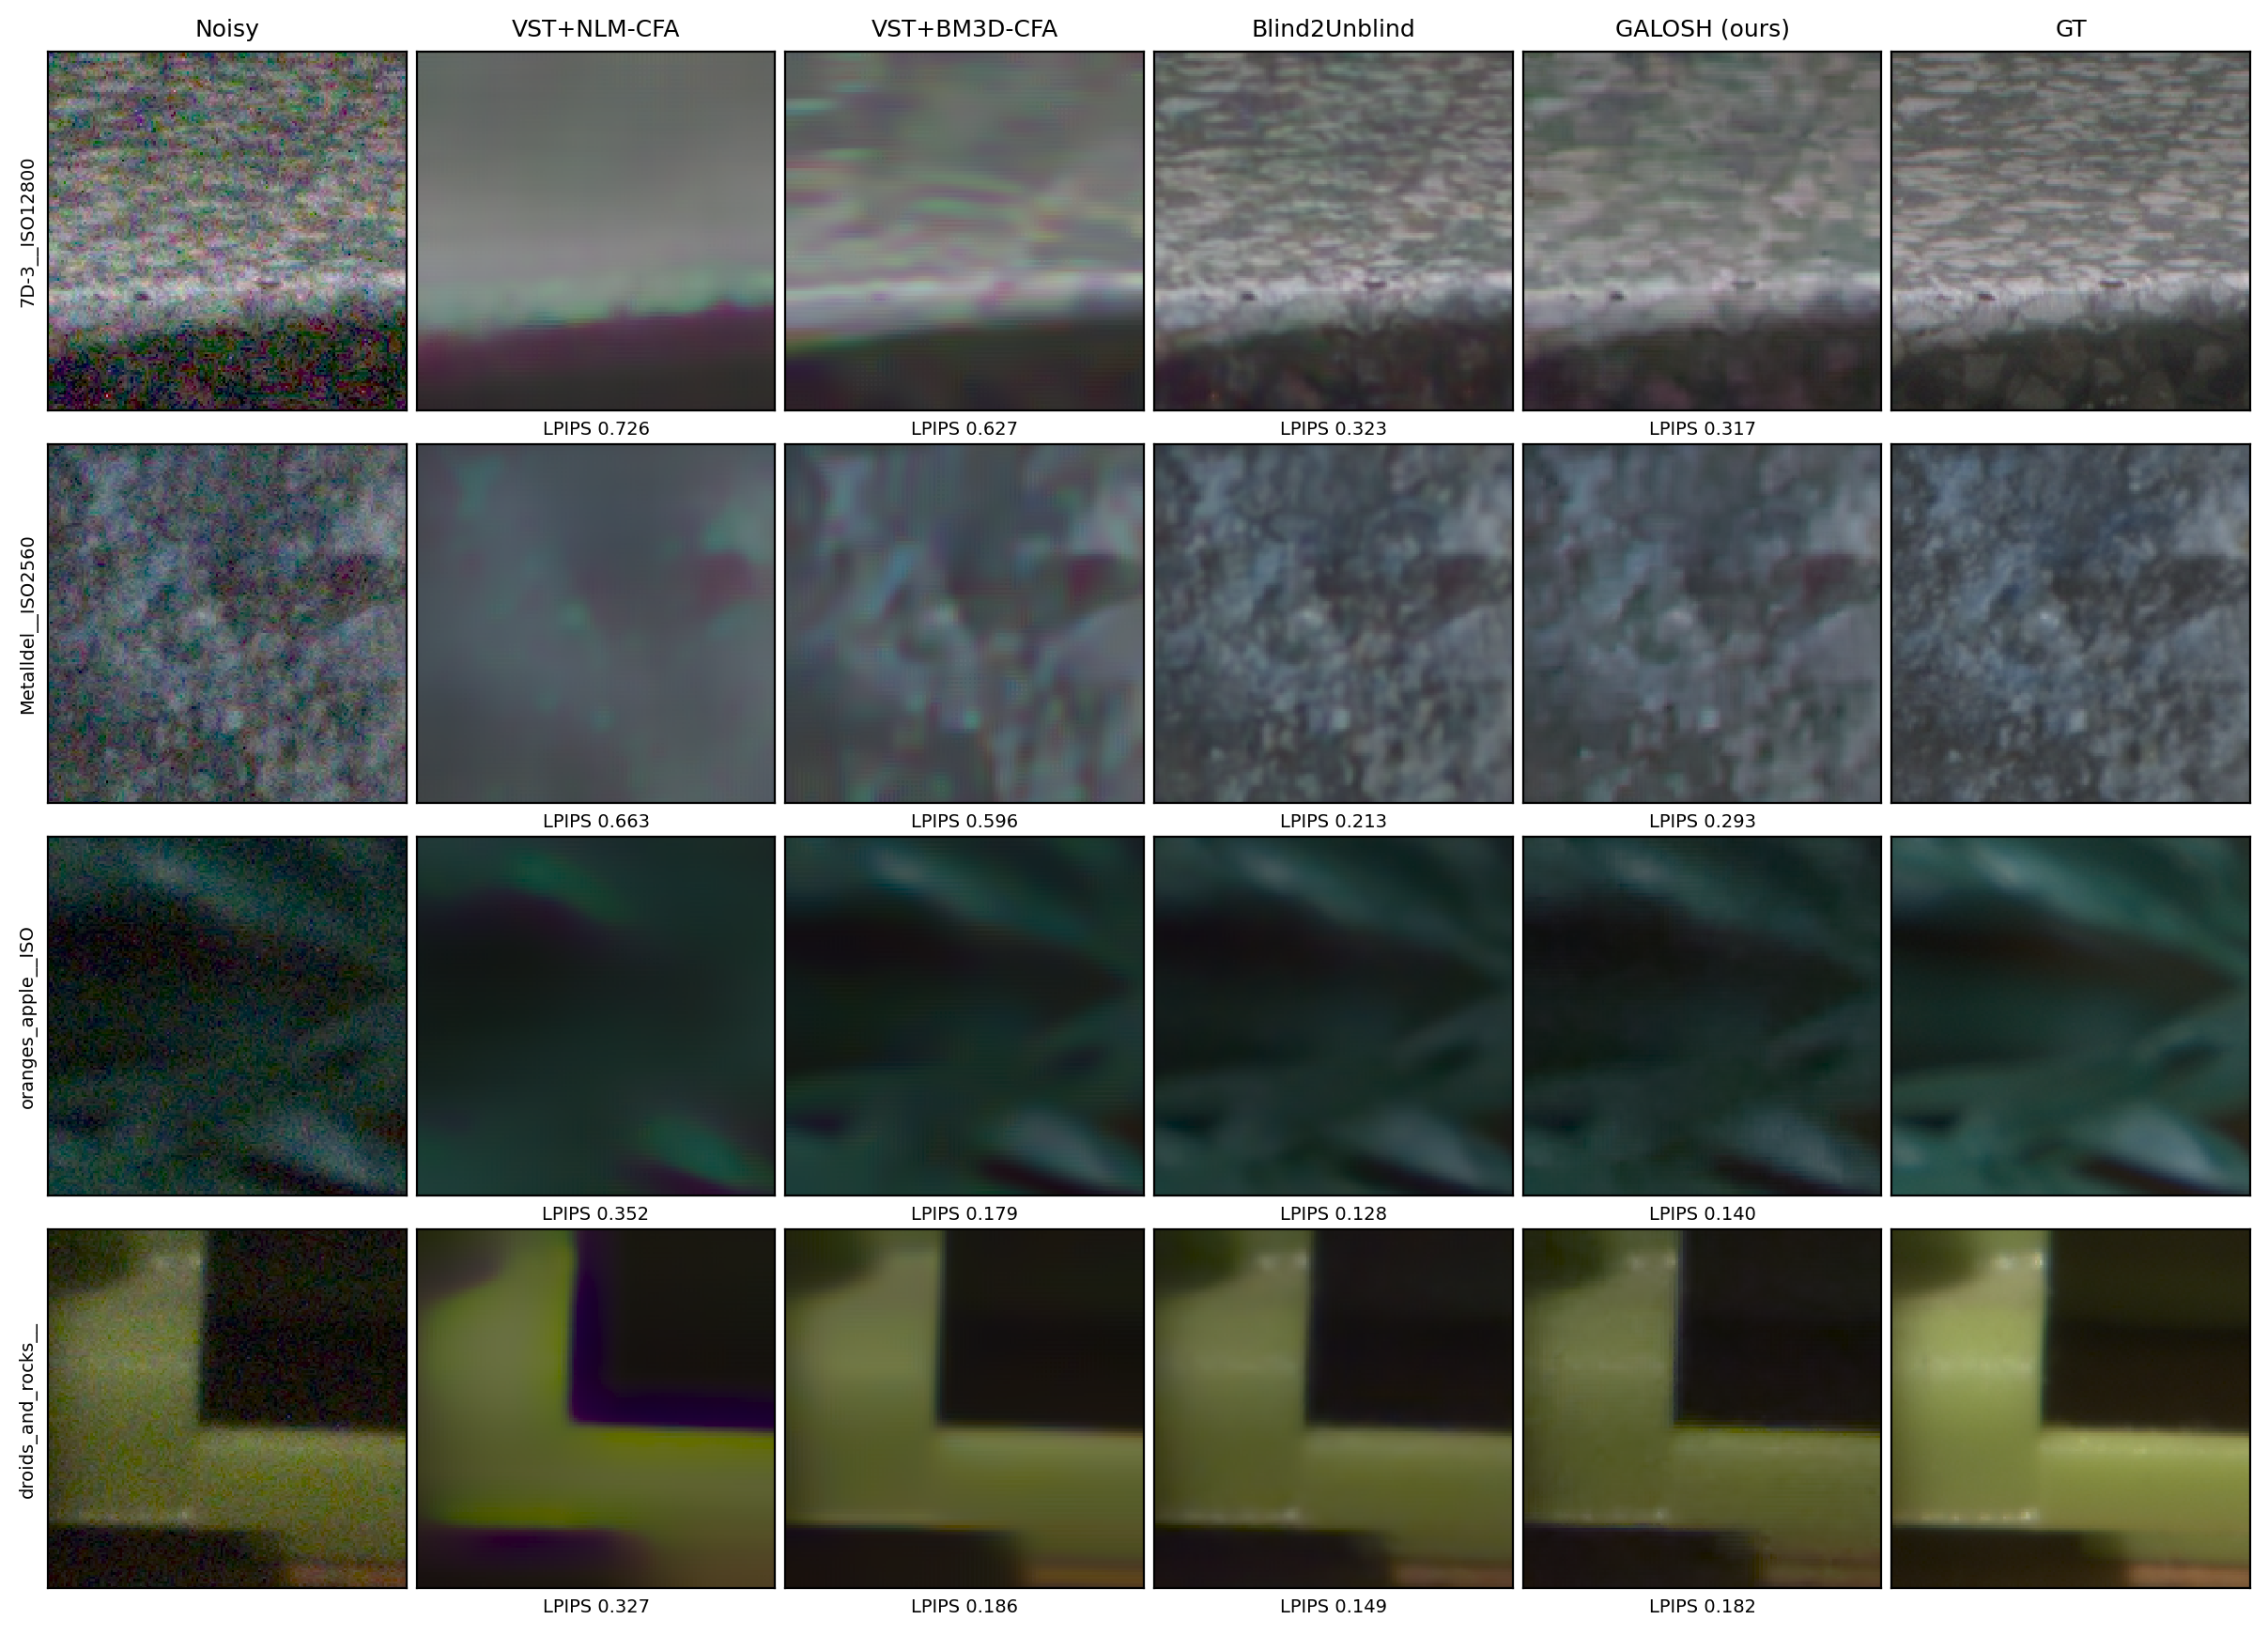
\includegraphics[width=0.92\textwidth]{../qualitative_rawnind.png}
\caption{Raw domain, RawNIND. Columns: Noisy / VST+NLM-CFA / VST+BM3D-CFA /
Blind2Unblind (trained) / \textbf{GALOSH (ours, blind)} / GT, with per-image
LPIPS ($\downarrow$). The classical baselines are given the noise-aware VST
front-end; GALOSH is fully blind.}
\label{fig:qual}
\end{figure*}

\begin{figure*}[t]
\centering

\includegraphics[width=0.92\textwidth]{../qualitative_srgb_sidd.png}
\caption{sRGB domain, SIDD Medium (full frame). Columns: Noisy / CBM3D /
Color-NLM / Guided / NAFNet-SIDD / SCUNet / Restormer-SIDD /
\textbf{GALOSH-YUV (ours)} / GT, with per-image LPIPS ($\downarrow$). All
methods blind; the classical baselines leave large residual noise on the
correlated rendering noise, and GALOSH sits between them and the SIDD-trained
networks.}
\label{fig:qualsrgb}
\end{figure*}

\begin{thebibliography}{21}\small
\bibitem{bm3d} K.~Dabov, A.~Foi, V.~Katkovnik, and K.~Egiazarian, ``Image
denoising by sparse 3-D transform-domain collaborative filtering,'' \emph{IEEE
TIP}, 2007.
\bibitem{nlm} A.~Buades, B.~Coll, and J.-M.~Morel, ``A non-local algorithm for
image denoising,'' \emph{CVPR}, 2005.
\bibitem{foi} A.~Foi, M.~Trimeche, V.~Katkovnik, and K.~Egiazarian,
``Practical Poissonian-Gaussian noise modeling and fitting for single-image
raw-data,'' \emph{IEEE TIP}, 2008.
\bibitem{makitalo} M.~Makitalo and A.~Foi, ``Optimal inversion of the
generalized Anscombe transformation for Poisson-Gaussian noise,'' \emph{IEEE
TIP}, 2013.
\bibitem{bayesshrink} S.~G.~Chang, B.~Yu, and M.~Vetterli, ``Adaptive wavelet
thresholding for image denoising and compression,'' \emph{IEEE TIP}, 2000.
\bibitem{loess} W.~S.~Cleveland, ``Robust locally weighted regression and
smoothing scatterplots,'' \emph{JASA}, 1979.
\bibitem{kopf} J.~Kopf, M.~F.~Cohen, D.~Lischinski, and M.~Uyttendaele,
``Joint bilateral upsampling,'' \emph{ACM SIGGRAPH}, 2007.
\bibitem{guidedfilter} K.~He, J.~Sun, and X.~Tang, ``Guided image filtering,''
\emph{ECCV}, 2010.
\bibitem{wnnm} S.~Gu, L.~Zhang, W.~Zuo, and X.~Feng, ``Weighted nuclear norm
minimization with application to image denoising,'' \emph{CVPR}, 2014.
\bibitem{epll} D.~Zoran and Y.~Weiss, ``From learning models of natural image
patches to whole image restoration,'' \emph{ICCV}, 2011.
\bibitem{ksvd} M.~Elad and M.~Aharon, ``Image denoising via sparse and
redundant representations over learned dictionaries,'' \emph{IEEE TIP}, 2006.
\bibitem{noiseclinic} M.~Lebrun, M.~Colom, and J.-M.~Morel, ``The noise
clinic: A blind image denoising algorithm,'' \emph{IPOL}, 2015.
\bibitem{b2u} Z.~Wang et al., ``Blind2Unblind: Self-supervised image denoising
with visible blind spots,'' \emph{CVPR}, 2022.
\bibitem{nafnet} L.~Chen, X.~Chu, X.~Zhang, and J.~Sun, ``Simple baselines for
image restoration,'' \emph{ECCV}, 2022.
\bibitem{restormer} S.~W.~Zamir et al., ``Restormer: Efficient transformer for
high-resolution image restoration,'' \emph{CVPR}, 2022.
\bibitem{scunet} K.~Zhang et al., ``Practical blind image denoising via
Swin-Conv-UNet and data synthesis,'' \emph{Machine Intelligence Research},
2023.
\bibitem{sidd} A.~Abdelhamed, S.~Lin, and M.~S.~Brown, ``A high-quality
denoising dataset for smartphone cameras,'' \emph{CVPR}, 2018.
\bibitem{rawnind} B.~Brummer and C.~De~Vleeschouwer, ``Natural image noise
dataset,'' \emph{CVPRW}, 2019.
\bibitem{lpips} R.~Zhang, P.~Isola, A.~A.~Efros, E.~Shechtman, and O.~Wang,
``The unreasonable effectiveness of deep features as a perceptual metric,''
\emph{CVPR}, 2018.
\bibitem{galosharxiv} Y.~Sato, ``GALOSH: Blind, training-free denoising of raw
Bayer and sRGB images by parallel-friendly local shrinkage,'' arXiv preprint,
2026. % TODO: insert arXiv ID (2507.XXXXX) when announced
\end{thebibliography}

\end{document}
